\chapter[Finite differences for parabolic problems]{Finite differences for \\
parabolic problems in 1D}
Consider the following \emph{initial-boundary value problem} for~$u=u(x,t)$,
\begin{equation}\label{eq: heat ivp 1d}
\begin{aligned}
u_t-au_{xx}&=f(x,t)&&\text{for $0<x<L$ and $0<t<T$,}\\
u&=\gamma_0(t)&&\text{at $x=0$, for $0<t<T$,}\\
u&=\gamma_L(t)&&\text{at $x=L$, for $0<t<T$,}\\
u&=u_0(x)&&\text{for $0<x<L$ when $t=0$,}
\end{aligned}
\end{equation}
where $u_t=\partial u/\partial t$ and $u_{xx}=\partial^2u/\partial x^2$.  For 
simplicity, we assume that the coefficient~$a$ is a positive constant.  The 
problem~\eqref{eq: heat ivp 1d} provides a model of heat conduction in 1D, 
where $u(x,t)$ is the temperature at position~$x$ and time~$t$.  The 
coefficient~$a>0$ is the \emph{thermal conductivity}: the value of~$a$ will be 
large for a material that conducts heat well, but small for a 
material that conducts heat poorly (that is, for a thermal insulator).  The 
\emph{source term}~$f(x,t)$ gives the density of any heat sources in the 
material, the \emph{boundary conditions} specify the temperatures $\gamma_0$~and 
$\gamma_L$ at the two edges of the spatial domain~$[0,L]$, and the 
\emph{initial condition} gives the temperature field~$u_0(x)$ when~$t=0$.  In 
this 1D model, the temperature does not vary in the $y$~and $z$ directions.

\section{Separation of variables}\label{sec: separation}

Let
\begin{equation}\label{eq: gamma(x,t)}
\gamma(x,t)=\frac{1}{L}\bigl((L-x)\gamma_0(t)+x\gamma_L(t)\bigr),
\end{equation}
so that
\[
\gamma(0,t)=\gamma_0(t)\quad\text{and}\quad\gamma(L,t)=\gamma_L(t),
\]
with
\[
\gamma_t-a\gamma_{xx}=\frac{1}{L}\bigl((L-x)\gamma_0'(t)+x\gamma_L'(t)\bigr).
\]
Thus, the difference $v=u-\gamma$ satisfies 
\begin{equation}\label{eq: heat ivp homog 1d}
\begin{aligned}
v_t-av_{xx}&=g(x,t)&&\text{for $0<x<L$ and $0<t<T$,}\\
v&=0&&\text{at $x=0$, for $0<t<T$,}\\
v&=0&&\text{at $x=L$, for $0<t<T$,}\\
v&=v_0(x)&&\text{for $0<x<L$ when $t=0$,}
\end{aligned}
\end{equation}
where 
\[
g(x,t)=f(x,t)-\gamma_t(x,t)
\quad\text{and}\quad
v_0(x)=u_0(x)-\gamma(x,0).
\]
In this way, it suffices to solve a problem with \emph{homogeneous} boundary 
conditions.


Associated with the time-dependent problem~\eqref{eq: heat ivp homog 1d} is the 
Sturm--Liouville \emph{eigenproblem},
\begin{equation}\label{eq: simple eigenproblem}
-a\phi''=\lambda\phi\quad\text{for $0<x<L$,}
	\quad\text{with $\phi(0)=0=\phi(L)$,}
\end{equation}
which has only the trivial solution~$\phi(x)\equiv0$ unless $\lambda$ is one of 
the \emph{eigenvalues} 
\[
\lambda_n=a\biggl(\frac{n\pi}{L}\biggr)^2\quad\text{for $n\in\{1,2,3,\ldots\}$.}
\]
When $\lambda=\lambda_n$, the solution~$\phi$ is a constant multiple of the 
corresponding \emph{eigenfunction}
\[
\phi_n(x)=\sin\frac{n\pi}{L}\,x.
\]
The eigenfunctions are \emph{orthogonal} with respect to the 
\emph{inner product}
\[
\langle f,g\rangle=\int_0^Lf(x)g(x)\,dx,
\]
that is,
\[
\langle\phi_n,\phi_k\rangle=0\quad\text{if $n\ne k$,}
\]
and their 2-norms are given by
\[
\|\phi_n\|^2=\langle\phi_n,\phi_n\rangle=\frac{L}{2}.
\]

Given a square-integrable function~$f(x)$, we define the 
\emph{Fourier sine coefficients}
\[
\hat f_n=\frac{\langle f,\phi_n\rangle}{\|\phi_n\|^2}
    =\frac{2}{L}\int_0^Lf(x)\sin\biggl(\frac{n\pi}{L}\,x\biggr)\,dx
    \quad\text{for $n\in\{1,2,3,\ldots\}$.}
\]
The \emph{completeness} of the eigenfunctions means that the Fourier sine series
\[
Sf(x)=\sum_{n=1}^\infty\hat f_n\sin\frac{n\pi}{L}\,x
\]
converges to~$f(x)$ in the \emph{mean-square sense}.  The Fourier coefficients 
of~$v(x,t)$ are functions of~$t$,
\[
\hat v_n(t)=\langle v(\cdot,t),\phi_n\rangle
    =\frac{2}{L}\int_0^Lv(x,t)\sin\biggl(\frac{n\pi}{L}\,x\biggr)\,dx,
\]
and formal term-by-term differentiation of the Fourier expansion of~$v$ gives
\[
v_t(x,t)=\frac{\partial}{\partial t}\sum_{n=1}^\infty\hat v_n(t)\phi_n(x)
    =\sum_{n=1}^\infty\frac{d\hat v_n}{dt}\,\phi_n(x).
\]
Since $\phi=\phi_n$ satisfies \eqref{eq: simple eigenproblem} 
with~$\lambda=\lambda_n$,
\[
-av_{xx}=-a\,\frac{\partial^2}{\partial x^2}
    \sum_{n=1}^\infty\hat v_n(t)\phi_n(x)
    =\sum_{n=1}^\infty\hat v_n(t)\bigl(-a\phi_n''(x)\bigr)
    =\sum_{n=1}^\infty\hat v_n(t)\bigl(\lambda_n\phi_n(x)\bigr),
\]
and so
\[
v_t-av_{xx}=\sum_{n=1}^\infty
	\biggl(\frac{d\hat v_n}{dt}+\lambda_n\hat v_n\biggr)\phi_n(x),
\]
which equals $g(x,t)$ if and only if all of the Fourier coefficients match, 
that is,
\[
\frac{d\hat v_n}{dt}+\lambda_n\hat v_n=\hat g_n(t)
    \quad\text{for $0<t<T$ and $n\in\{1,2,3,\ldots\}$.}
\]
Multiplying both sides of this linear, first-order ODE by the 
\emph{integrating factor}~$e^{\lambda_n t}$ we obtain
\[
e^{\lambda_nt}\,\frac{d\hat v_n}{dt}+\lambda_ne^{\lambda_nt}\hat v_n
	=e^{\lambda_nt}\hat g_n(t),
\]
and since the left-hand side equals $(d/dt)(e^{\lambda_nt}\hat v_n)$ it 
follows that
\[
e^{\lambda_nt}\hat v_n(t)-\hat v_n(0)=\int_0^te^{\lambda_ns}\hat g_n(s)\,ds.
\]
Thus,
\begin{equation}\label{eq: Duhamel n}
\hat v_n(t)=\hat v_n(0)e^{-\lambda_nt}
	+\int_0^te^{-\lambda_n(t-s)}\hat g_n(s)\,ds\quad\text{for $t\ge0$,}
\end{equation}
and multiplying both sides by~$\phi_n(x)$ and summing over~$n$, we obtain the
series representation
\[
v(x,t)=\sum_{n=1}^\infty\hat v_n(t)\phi_n(x)
	=\sum_{n=1}^\infty e^{-\lambda_nt}\hat v_n(0)\phi_n(x)
	+\int_0^t\sum_{n=1}^\infty e^{-\lambda_n(t-s)}\hat g_n(s)\phi_n(x)\,ds.
\]

Define the differential operator~$\mathcal{A}v=-v''$ so that 
$\mathcal{A}\phi_n=\lambda_n\phi_n$, and then define the linear 
operator~$e^{-t\mathcal{A}}$ by
\[
(e^{-t\mathcal{A}}v)(x)=\sum_{n=1}^\infty e^{-\lambda_nt}\hat v_n\phi_n(x).
\]
In particular, this definition means that
\[
e^{-t\mathcal{A}}\phi_n=e^{-\lambda_nt}\phi_n
	\quad\text{for $n\in\{1,2,3,\ldots\}$,}
\]
and
\[
\sum_{n=1}^\infty e^{-\lambda_nt}\hat v_n(0)\phi_n(x)=e^{-t\mathcal{A}}v_0(x)
\]
with
\[
\sum_{n=1}^\infty e^{-\lambda_n(t-s)}\hat g_n(s)\phi_n(x)
	=e^{-(t-s)\mathcal{A}}g(x,s),
\]
so \eqref{eq: Duhamel n} can be written more succinctly as
\[
v(x,t)=e^{-t\mathcal{A}}v_0(x)+\int_0^te^{-(t-s)\mathcal{A}}g(x,s)\,ds.
\]
This representation of~$v$ is known as the \emph{Duhamel formula}, and the 
solution of our original problem~\eqref{eq: heat ivp 1d} is then given by
\[
u(x,t)=\gamma(x,t)+v(x,t)\quad\text{for $0\le x\le L$ and $0\le t\le T$.}
\]

\section{Semidiscrete method}

We define a uniform grid on the spatial interval~$[0,L]$,
\[
x_p=p\,\Delta x\quad\text{for $0\le p\le P$,}
	\quad\text{with $\Delta x=\frac{L}{P}$,}
\]
and let
\[
U_p(t)\approx u(x_p,t),\qquad f_p(t)=f(x_p,t),\qquad u_{0p}=u_0(x_p).
\]
Since $u_t(x_p,t)\approx dU_p/dt$ and
\[
u_{xx}(x_p,t)\approx\frac{u(x_{p+1},t)-2u(x_p,t)+u(x_{p-1},t)}{\Delta x^2}
	\approx\frac{U_{p+1}(t)-2U_p(t)+U_{p-1}(t)}{\Delta x^2},
\]
we formulate the following semidiscrete approximation to the initial-boundary 
value problem~\eqref{eq: heat ivp 1d},
\begin{equation}\label{eq: semidiscrete heat 1d}
\begin{aligned}
\frac{dU_p}{dt}-a\,\frac{U_{p+1}-2U_p+U_{p-1}}{\Delta x^2}&=f_p(t)&
	&\text{for $1\le p\le P-1$ and $0<t<T$,}\\
U_0&=\gamma_0(t)&&\text{for $0<t<T$,}\\
U_P&=\gamma_P(t)&&\text{for $0<t<T$,}\\
U_p&=u_{0p}&&\text{for $1\le p\le P-1$ when $t=0$.}
\end{aligned}
\end{equation}
This system can be written in matrix-vector notation as
\begin{equation}\label{eq: ODE system}
\frac{d\boldsymbol{U}}{dt}+\boldsymbol{A}\boldsymbol{U}=\boldsymbol{f}(t)
	+\boldsymbol{g}(t),
\end{equation}
where
\[
\boldsymbol{A}=\frac{a}{\Delta x^2}\begin{bmatrix}
 2&    -1&      &      &\\
-1&     2&    -1&      &\\
  &\ddots&\ddots&\ddots&\\
  &      &    -1&     2&-1\\
  &      &      &    -1& 2\end{bmatrix},\qquad
\]
and
\begin{equation}\label{eq: U f g semidiscrete 1d}
\boldsymbol{U}(t)=\begin{bmatrix}
U_1(t)\\ U_2(t)\\ \vdots\\ U_{P-2}(t)\\ U_{P-1}(t)\end{bmatrix},\qquad
\boldsymbol{f}(t)=\begin{bmatrix}
f_1(t)\\ f_2(t)\\ \vdots\\ f_{P-2}(t)\\ f_{P-1}(t)\end{bmatrix},\qquad
\boldsymbol{g}(t)=\frac{a}{\Delta x^2}\begin{bmatrix}
\gamma_0(t)\\ 0\\ \vdots\\ 0\\ \gamma_L(t)\end{bmatrix}.
\end{equation}
Recall that for any square matrix~$\boldsymbol{A}$, the matrix exponential
is defined by the convergent infinite series
\[
e^{\boldsymbol{A}}=\sum_{k=0}^\infty\frac{\boldsymbol{A}^n}{n!}
	=\boldsymbol{I}+\boldsymbol{A}+\frac{\boldsymbol{A}^2}{2!}
	+\frac{\boldsymbol{A}^3}{3!}+\cdots.
\]
Furthermore,
\[
\frac{d}{dt}\,e^{t\boldsymbol{A}}=\boldsymbol{A}e^{t\boldsymbol{A}}
	=e^{t\boldsymbol{A}}\boldsymbol{A},
\]
so $e^{t\boldsymbol{A}}$ provides an integrating factor 
for~\eqref{eq: ODE system}:
\[
\frac{d}{dt}\bigl(e^{t\boldsymbol{A}}\boldsymbol{U}\bigr)
	=e^{t\boldsymbol{A}}\boldsymbol{A}\boldsymbol{U}
	+e^{t\boldsymbol{A}}\,\frac{d\boldsymbol{U}}{dt}
	=e^{t\boldsymbol{A}}\biggl(\frac{d\boldsymbol{U}}{dt}
	+\boldsymbol{A}\boldsymbol{U}\biggr)
	=e^{t\boldsymbol{A}}\bigl(\boldsymbol{f}(t)+\boldsymbol{g}(t)\bigr).
\]
If $t=0$ then $e^{t\boldsymbol{A}}=\boldsymbol{I}$ is the identity matrix, so
\[
e^{t\boldsymbol{A}}\boldsymbol{U}(t)-\boldsymbol{U}(0)
	=\int_0^te^{s\boldsymbol{A}}\bigl(
		\boldsymbol{f}(s)+\boldsymbol{g}(s)\bigr)\,ds.
\]
Using $e^{-t\boldsymbol{A}}=(e^{t\boldsymbol{A}})^{-1}$~and 
$e^{-t\boldsymbol{A}}e^{s\boldsymbol{A}}=e^{-(t-s)\boldsymbol{A}}$, we obtain
a semidiscrete Duhamel formula,
\[
\boldsymbol{U}(t)=e^{-t\boldsymbol{A}}\boldsymbol{u}_0
	+\int_0^te^{-(t-s)\boldsymbol{A}}\bigl(
		\boldsymbol{f}(s)+\boldsymbol{g}(s)\bigr)\,ds,
\]
where $\boldsymbol{u}_0=[u_0(x_p)]_{p=1}^{P-1}$ is the vector of initial data.

\section{Explicit Euler method}

To obtain a fully-discrete scheme, we introduce a uniform grid on the time axis,
\[
t_n=n\,\Delta t\quad\text{for $0\le n\le N$,}
	\quad\text{where $\Delta t=\frac{T}{N}$,}
\]
and let
\[
U^n_p\approx u(x_p,t_n),\quad
f^n_p=f(x_p,t_n),\quad
\gamma_0^n=\gamma_0(t_n),\quad
\gamma_L^n=\gamma_L(t_n),\quad
u_{0p}=u_0(x_p).
\]
The \emph{forward difference} approximation in time,
\[
u_t(x_p,t_n)\approx\frac{u(x_p,t_n+\Delta t)-u(x_p,t_n)}{\Delta t}
	=\frac{u(x_p,t_{n+1})-u(x_p,t_n)}{\Delta t}
		\approx\frac{U^{n+1}_p-U^n_p}{\Delta t},
\]
and the second-order central difference approximation in space,
\begin{align*}
u_{xx}(x_p,t_n)
&\approx\frac{u(x_p+\Delta x,t_n)-2u(x_p,t_n)+u(x_p-\Delta x,t_n)}{\Delta x^2}\\
&=\frac{u(x_{p+1},t_n)-2u(x_p,t_n)+u(x_{p-1},t_n)}{\Delta x^2}
\approx\frac{U^n_{p+1}-2U^n_p+U^n_{p-1}}{\Delta x^2},
\end{align*}
lead to the \emph{explicit Euler method} for~\eqref{eq: heat ivp 1d}:
\begin{equation}\label{eq: explicit Euler 1d}
\begin{aligned}
\frac{U^{n+1}_p-U^n_p}{\Delta t}
	-a\,\frac{U^n_{p+1}-2U^n_p+U^n_{p-1}}{\Delta x^2}&=f^n_p&
&\text{for $1\le p\le P-1$ and $0\le n\le N-1$,}\\
U^n_0&=\gamma_0^n&&\text{for $0\le n\le N$,}\\
U^n_P&=\gamma_L^n&&\text{for $0\le n\le N$,}\\
U^0_p&=u_{0p}&&\text{for $1\le p\le P-1$.}
\end{aligned}
\end{equation}
We multiply both sides of the finite difference equation by~$\Delta t$ and put
\begin{equation}\label{eq: rho explicit Euler}
\rho=\frac{a\,\Delta t}{\Delta x^2}
\end{equation}
to obtain
\[
U^{n+1}_p-U^n_p-\rho(U^n_{p+1}-2U^n_p+U^n_{p-1})=f^n_p\,\Delta t
\]
and thus
\begin{equation}\label{eq: explicit Euler stencil}
U^{n+1}_p=f^n_p\,\Delta t+\rho U^n_{p-1}+(1-2\rho)U^n_p+\rho U^n_{p+1}.
\end{equation}
In this way, the scheme provides an \emph{explicit} formula for the solution 
at~$(x_p,t_{n+1})$ given the values at the three nearest grid 
points $(x_{p-1},t_n)$, $(x_p,t_n)$~and $(x_{p+1},t_n)$ from the previous time 
level.  We say the these four points constitute the \emph{stencil} for the 
method; see \cref{fig: explicit Euler stencil}.
\cref{alg: explicit Euler} shows how the 
formula~\eqref{eq: explicit Euler stencil} is used to compute the finite 
difference solution~$U^n_p$ by advancing from one time level to the next, 
starting at~$t_0=0$.  

\begin{figure}
\caption{Computational stencil for the explicit Euler 
method~\eqref{eq: explicit Euler stencil}.}
\label{fig: explicit Euler stencil}
\begin{center}
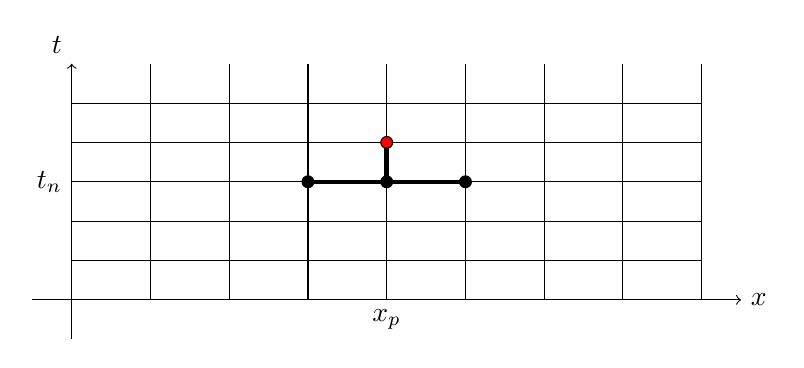
\begin{tikzpicture}[scale=0.5]
\draw[->] (-1,0) -- (17,0);
\node[right] at (17,0) {$x$};
\node[below] at (8,0) {$x_p$};
\draw[->] (0,-1) -- (0,6);
\node[above left] at (0,6) {$t$};
\node[left] at (0,3) {$t_n$};
\foreach \x in {2, 4, ..., 16}
    \draw[thin] (\x,0) -- (\x,6);
\foreach \y in {1, ..., 5}
    \draw[thin] (0,\y) -- (16,\y);
\draw[ultra thick] (6,3) -- (8,3) -- (10,3);
\draw[fill] (6,3)  circle (0.15cm);
\draw[fill] (8,3)  circle (0.15cm);
\draw[fill] (10,3) circle (0.15cm);
\draw[ultra thick] (8,3) -- (8,4);
\draw[fill=red] (8,4)  circle (0.15cm);
\end{tikzpicture}
\end{center}
\end{figure}

\begin{algorithm}
\caption{Explicit Euler method.}
\label{alg: explicit Euler}
\begin{algorithmic}
\State Allocate storage for $x_p$, $t_n$~and $U^n_p$, where $0\le p\le P$ and 
$0\le n\le N$.
\State $\Delta x=L/P$ 
\State$\Delta t=T/N$
\For{$p=0:P$}
    \State $x_p=p\,\Delta x$
\EndFor
\For{$n=0:N$}
    \State $t_n=n\,\Delta t$
    \State $U^n_0=\gamma_0^n$
    \State $U^n_P=\gamma_L^n$
\EndFor
\State $\rho=a\,\Delta t/\Delta x^2$
\For{$p=1:P-1$}
    \State $U^0_p=u_0(x_p)$
\EndFor
\For{$n=0:N-1$}
    \For{$p=1:P-1$}
        \State $U^{n+1}_p=f^n_p\,\Delta t
                +\rho U^n_{p-1}+(1-2\rho)U^n_p+\rho U^n_{p+1}$
    \EndFor                
\EndFor
\end{algorithmic}
\end{algorithm}

We now show that the explicit Euler method is stable provided the time 
step~$\Delta t$ is sufficiently small compared to the spatial grid 
size~$\Delta x$.

\begin{theorem}\label{thm: explicit Euler stability}
If $\Delta x$ and $\Delta t$ satisfy
\begin{equation}\label{eq: explicit Euler timestep}
\Delta t\le\frac{\Delta x^2}{2a},                                        
\end{equation}
or equivalently if the ratio~\eqref{eq: rho explicit Euler} satisfies 
$\rho\le1/2$, then the explicit Euler method~\eqref{eq: explicit Euler 1d} is 
stable:
\begin{equation}\label{eq: explicit Euler stability}
\|\boldsymbol{U}^n_{0:P}\|_\infty
	\le\max\bigl\{\|(\boldsymbol{u}_0)_{1:P-1}\|_\infty, 
		\|\gamma_0^{0:n}\|_\infty,\|\gamma_L^{0:n}\|_\infty\bigr\}
	+\sum_{j=0}^{n-1}\|\boldsymbol{f}^j_{1:P-1}\|_\infty\,\Delta t
\end{equation}
for $0\le n\le N$.
\end{theorem}
\begin{proof}
We use finite induction on~$n$.  When~$n=0$, we have
$U^0_p=u_{0p}$ for~$1\le p\le P-1$, with $U^0_0=\gamma_0^0$~and 
$U^0_P=\gamma_L^0$, so 
\[
\|\boldsymbol{U}^0_{0:P}\|_\infty=
\max\bigl\{\|(\boldsymbol{u}_0)_{1:P-1}\|_\infty,|\gamma_0|,|\gamma_L|\bigr\},
\]
which agrees with the formula since the empty sum vanishes. Now let 
$0\le n\le N-1$ and make the induction
hypothesis~\eqref{eq: explicit Euler stability}.  We see
from~\eqref{eq: explicit Euler stencil} that, for $1\le p\le P-1$,
\[
|U^{n+1}_p|\le|f^n_p|\,\Delta t+\rho|U^n_{p-1}|+|1-2\rho|\,|U^n_p|
    +\rho|U^n_{p+1}|
\]
and thus
\[
|U^{n+1}_p|\le\|\boldsymbol{f}^n_{1:P-1}\|_\infty\,\Delta t
		+(2\rho+|1-2\rho|)\|\boldsymbol{U}^n_{0:P}\|_\infty
\quad\text{for $1\le p\le P-1$.} 
\]
If $\rho\le1/2$, then $2\rho+|1-2\rho|=2\rho+1-2\rho=1$ so
\begin{align*}
\|\boldsymbol{U}^{n+1}_{1:P-1}\|_\infty
	&\le\|\boldsymbol{U}^n_{0:P}\|_\infty
		+\|\boldsymbol{f}^n_{1:P-1}\|_\infty\,\Delta t\\
	&\le\max\bigl\{\|(\boldsymbol{u}_0)_{1:P-1}\|_\infty, 
		\|\gamma_0^{0:n}\|_\infty,\|\gamma_L^{0:n}\|_\infty\bigr\}
	+\sum_{j=0}^{n-1}\|\boldsymbol{f}^j_{1:P-1}\|_\infty\,\Delta t
		+\|\boldsymbol{f}^n_{1:P-1}\|_\infty\,\Delta t\\
	&=\max\bigl\{\|(\boldsymbol{u}_0)_{1:P-1}\|_\infty, 
		\|\gamma_0^{0:n}\|_\infty,\|\gamma_L^{0:n}\|_\infty\bigr\}
	+\sum_{j=0}^n\|\boldsymbol{f}^j_{1:P-1}\|_\infty\,\Delta t,
\end{align*}
and since $U^{n+1}_0=\gamma_0^{n+1}$~and $U^{n+1}_P=\gamma_L^{n+1}$
\[
\|\boldsymbol{U}^{n+1}_{0:P}\|_\infty
	\le\max\bigl\{\|(\boldsymbol{u}_0)_{1:P-1}\|_\infty, 
		\|\gamma_0^{0:n+1}\|_\infty,\|\gamma_L^{0:n+1}\|_\infty\bigr\}
	+\sum_{j=0}^n\|\boldsymbol{f}^j_{1:P-1}\|_\infty\,\Delta t,
\]
as required.
\end{proof}

The \emph{local trunction error} for the explicit Euler method is defined by
\begin{equation}\label{eq: tau explicit Euler}
\tau(x,t)=f(x,t)-\frac{u(x,t+\Delta t)-u(x,t)}{\Delta t}
	+a\,\frac{u(x+\Delta x,t)-2u(x,t)+u(x-\Delta x,t)}{\Delta x^2},
\end{equation}
and measures the extent to which the solution~$u(x,t)$ of the continuous 
problem~\eqref{eq: heat ivp 1d} fails to satisfy the finite difference equation.
We can estimate $\tau^n_p=\tau(x_p,t_n)$ by Taylor expansion.

\begin{lemma}\label{lem: tau explicit Euler}
If $u_{tt}$~and $u_{xxxx}$ are continuous for~$(x,t)\in[0,L]\times[0,T]$, then
\[
|\tau^n_p|\le\frac{\Delta t}{2}\max_{[0,L]\times[0,T]}|u_{tt}|
	+a\,\frac{\Delta x^2}{12}\max_{[0,L]\times[0,T]}|u_{xxxx}|
\]
for $1\le p\le P-1$ and $0\le n\le N-1$.
\end{lemma}
\begin{proof}
Since $u_t-au_{xx}=f$,
\[
|\tau(x,t)|=\biggl|u_t-\frac{u(x,t+\Delta t)-u(x,t)}{\Delta t}
	-a\biggl(u_{xx}-\frac{u(x+\Delta x,t)-2u(x,t)+u(x-\Delta x,t)}{\Delta x^2}
\biggr)\biggr|,
\]
and, so by Exercise~\ref{ex: forward diff}~and \cref{thm: 2nd central diff},
\[
|\tau(x,t)|\le\frac{\Delta t}{2}\max_{t\le s\le t+\Delta t}|u_{tt}(x,s)|
	+a\,\frac{\Delta x^2}{12}\,
	\max_{x-\Delta x\le y\le x+\Delta x}|u_{xxxx}(y,t)|,
\]
which implies the stated estimate for~$\tau^n_p$. 
\end{proof}

We can now deduce that, provided the
restriction~\eqref{eq: explicit Euler timestep} on the step sizes is satisfied,
the explicit Euler method is first-order accurate in time and second-order 
accurate in space.

\begin{theorem}\label{thm: explicit Euler error}
Assume that $\Delta x$~and $\Delta t$ satisfy 
\eqref{eq: explicit Euler timestep}, and that $u_{tt}$~and $u_{xxxx}$ are 
continuous on~$[0,L]\times[0,T]$. Then the error for the explicit Euler method 
satisfies
\[
|U^n_p-u(x_p,t_n)|\le Ct_n(\Delta t+\Delta x^2)
\quad\text{for $0\le p\le P-1$ and $0\le n\le N$,}
\]
where
\begin{equation}\label{eq: error const explicit Euler}
C=\max\biggl(\frac{1}{2}\max_{[0,L]\times[0,T]}|u_{tt}|,
	\frac{1}{12}\max_{[0,L]\times[0,T]}|u_{xxxx}|\biggr).
\end{equation}
\end{theorem}
\begin{proof}
By the definition~\eqref{eq: tau explicit Euler} of the local truncation error,
\[
\frac{u(x_p,t_{n+1})-u(x_p,t_n)}{\Delta t}
	-a\,\frac{u(x_{p+1},t)-2u(x_p,t_n)+u(x_{p-1},t_n)}{\Delta x^2}
	=f^n_p-\tau^n_p.
\]
Subtracting this equation from the finite difference equation 
in~\eqref{eq: explicit Euler 1d}, we obtain a finite difference equation for
the error ~$E^n_p=U^n_p-u(x_p,t_n)$,
\[
\frac{E^{n+1}_p-E^n_p}{\Delta t}
	-a\,\frac{E^n_{p+1}-2E^n_p+E^n_{p-1}}{\Delta x^2}=\tau^n_p
\quad\text{for $1\le p\le P-1$ and $0\le n\le N-1$.}
\]
In addition, the boundary and initial conditions satisfied by $U^n_p$~and $u$ 
imply that
\[
\begin{aligned}
E^n_0&=U^n_0-u(x_0,t_n)=\gamma_0^n-\gamma_0^n=0&&\text{for $0\le n\le N$,}\\
E^n_P&=U^n_P-u(x_P,t_n)=\gamma_L^n-\gamma_L^n=0&&\text{for $0\le n\le N$,}\\
E^0_p&=U^0_p-u(x_p,t_0)=u_0(x_p)-u_0(x_p)=0&&\text{for $1\le p\le P-1$.}
\end{aligned}
\]
Thus, $E^n_p$ is the explicit Euler solution obtained when $f^n_p$, 
$\gamma_0^n$, $\gamma_L^n$~and $u_{0p}$ are replaced by $\tau^n_p$, $0$, 
$0$~and $0$, respectively.  The restriction on the step sizes allows us to apply 
the stability estimate of \cref{thm: explicit Euler stability} to deduce 
that
\[
\|\boldsymbol{E}^n_{0:P}\|_\infty
	\le\sum_{j=0}^{n-1}\|\boldsymbol{\tau}^n_{1:P-1}\|_\infty\,\Delta t
	\quad\text{for $0\le n\le N$.}
\]
By Lemma~\ref{lem: tau explicit Euler}, 
$\|\boldsymbol{\tau}^n_{1:P-1}\|_\infty\le C(\Delta t+\Delta x^2)$, so
\[
\|\boldsymbol{E}^n_{0:P}\|_\infty\le Cn(\Delta t+\Delta x^2)\,\Delta t
	=Ct_n(\Delta t+\Delta x^2),
\]
as claimed.
\end{proof}

\section{Implicit Euler method}

Instead of using a forward difference, we can approximate $u_t$ by a 
\emph{backward difference},
\[
u_t(x_p,t_n)\approx\frac{u(x_p,t_n)-u(x_p,t_n-\Delta t)}{\Delta t}
	=\frac{u(x_p,t_n)-u(x_p,t_{n-1})}{\Delta t}
	\approx\frac{U^n_p-U^{n-1}_p}{\Delta t},
\]
which leads to the \emph{im}plicit Euler method,
\begin{equation}\label{eq: implicit Euler 1d}
\begin{aligned}
\frac{U^n_p-U^{n-1}_p}{\Delta t}
	-a\,\frac{U^n_{p+1}-2U^n_p+U^n_{p-1}}{\Delta x^2}&=f^n_p&
&\text{for $1\le p\le P-1$ and $1\le n\le N$,}\\
U^n_0&=\gamma_0^n&&\text{for $0\le n\le N$,}\\
U^n_P&=\gamma_L^n&&\text{for $0\le n\le N$,}\\
U^0_p&=u_{0p}&&\text{for $1\le p\le P-1$.}
\end{aligned}
\end{equation}
Multiplying both sides of the finite difference equation by~$\Delta t$, and 
defining $\rho$ as before in~\eqref{eq: rho explicit Euler}, we obtain
\[
U^n_p-U^{n-1}_p-\rho(U^n_{p+1}-2U^n_p+U^n_{p-1})=f^n_p\,\Delta t
\]
and thus
\begin{equation}\label{eq: implicit Euler stencil}
-\rho U^n_{p-1}+(1+2\rho)U^n_p-\rho U^n_{p+1}=U^{n-1}_p+f^n_p\,\Delta t
\end{equation}
for $1\le p\le P-1$ and $1\le n\le N$.  Thus, at the $n$th time level we have a 
system of linear equations for the unknown $U^n_1$, $U^n_2$, \dots, $U^n_{P-1}$,
with the right-hand sides involving the solution at the previous time level.
The stencil for this scheme is shown in \cref{fig: implicit Euler stencil}.

\begin{figure}
\caption{Computational stencil for the implicit Euler 
method~\eqref{eq: implicit Euler stencil}.}
\label{fig: implicit Euler stencil}
\begin{center}
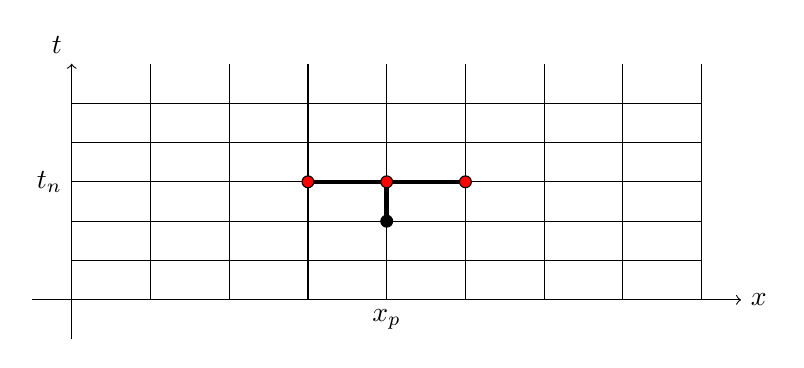
\begin{tikzpicture}[scale=0.5]
\draw[->] (-1,0) -- (17,0);
\node[right] at (17,0) {$x$};
\node[below] at (8,0) {$x_p$};
\draw[->] (0,-1) -- (0,6);
\node[above left] at (0,6) {$t$};
\node[left] at (0,3) {$t_n$};
\foreach \x in {2, 4, ..., 16}
    \draw[thin] (\x,0) -- (\x,6);
\foreach \y in {1, ..., 5}
    \draw[thin] (0,\y) -- (16,\y);
\draw[ultra thick] (8,2) -- (8,3);
\draw[fill] (8,2)  circle (0.15cm);
\draw[ultra thick] (6,3) -- (8,3) -- (10,3);
\draw[fill=red] (6,3)  circle (0.15cm);
\draw[fill=red] (8,3)  circle (0.15cm);
\draw[fill=red] (10,3) circle (0.15cm);
\end{tikzpicture}
\end{center}
\end{figure}

Equivalently, we can start from the matrix form of the semidiscrete
method~\eqref{eq: ODE system}, and approximate $d\boldsymbol{U}/dt$ with a 
backward difference to obtain
\begin{equation}\label{eq: implicit Euler 1d vector}
\frac{\boldsymbol{U}^n-\boldsymbol{U}^{n-1}}{\Delta t}
	+\boldsymbol{A}\boldsymbol{U}^n=\boldsymbol{f}^n+\boldsymbol{g}^n
\quad\text{for $1\le n\le N$,}
\end{equation}
where
\[
\boldsymbol{A}=\frac{a}{\Delta x^2}\begin{bmatrix}
 2&    -1&      &      &\\
-1&     2&    -1&      &\\
  &\ddots&\ddots&\ddots&\\
  &      &    -1&     2&-1\\
  &      &      &    -1& 2\end{bmatrix},\qquad
\]
and
\[
\boldsymbol{U}^n=\begin{bmatrix}
U^n_1\\ U^n_2\\ \vdots\\ U^n_{P-2}\\ U^n_{P-1}\end{bmatrix},\qquad
\boldsymbol{f}^n=\begin{bmatrix}
f^n_1\\ f^n_2\\ \vdots\\ f^n_{P-2}\\ f^n_{P-1}\end{bmatrix},\qquad
\boldsymbol{g}^n=\frac{a}{\Delta x^2}\begin{bmatrix}
\gamma_0^n\\ 0\\ \vdots\\ 0\\ \gamma_L^n\end{bmatrix}.
\]
Rearranging \eqref{eq: implicit Euler 1d vector} we find that
\[
(\boldsymbol{I}+\Delta t\,\boldsymbol{A})\boldsymbol{U}^n
	=\boldsymbol{U}^{n-1}+\Delta t\,(\boldsymbol{f}^n+\boldsymbol{g}^n)
\quad\text{for $1\le n\le N$.}
\]
Here, the coefficient matrix is symmetric, tridiagonal and positive-definite, 
so we can compute~$\boldsymbol{U}^n$ via a factorization
\[
\boldsymbol{I}+\Delta t\,\boldsymbol{A}
	=\boldsymbol{L}^T\boldsymbol{D}\boldsymbol{L},
\]
as shown in \cref{alg: implicit Euler}.

\begin{algorithm}
\caption{Implicit Euler method.}
\label{alg: implicit Euler}
\begin{algorithmic}
\State Allocate storage for $x_p$, $t_n$~and $U^n_p$, where $0\le p\le P$ and 
$0\le n\le N$.
\State Allocate storage for vectors $[d_1,d_2,\ldots,d_{P-1}]^T$~and
$[\ell_1,\ell_2,\ldots,\ell_{P-2}]^T$.
\State $\Delta x=L/P$ 
\State$\Delta t=T/N$
\For{$p=0:P$}
    \State $x_p=p\,\Delta x$
\EndFor
\For{$n=0:N$}
    \State $t_n=n\,\Delta t$
    \State $U^n_0=\gamma_0^n$
    \State $U^n_P=\gamma_L^n$
\EndFor
\State $\rho=a\,\Delta t/\Delta x^2$
\For{$p=1:P-1$}
    \State $d_p=1+2\rho$
\EndFor
\For{$p=1:P-2$}
    \State $\ell_p=-\rho$
\EndFor
\State \textsc{Factorize!}($\boldsymbol{d}$, $\boldsymbol{\ell}$)
\Comment Use \cref{alg: LDLT in place} to compute
$\boldsymbol{I}+\Delta t\,\boldsymbol{A}=\boldsymbol{L}\boldsymbol{D}
\boldsymbol{L}^T$ in place.
\For{$p=1:P-1$}
    \State $U^0_p=u_0(x_p)$
\EndFor
\For{$n=1:N$}
    \For{$p=1:P-1$}
        \State $U^n_p\gets U^{n-1}_p+\Delta t\,f(x_p,t_n)$
    \EndFor
    \State $U^n_1\gets U^n_1+a\gamma_0/\Delta x^2$
    \State $U^n_{P-1}\gets U^n_{P-1}+a\gamma_L/\Delta x^2$
    \State \textsc{Solve}!($\boldsymbol{U}^n_{1:P-1}$,
$\boldsymbol{d}$, $\boldsymbol{\ell}$)
\Comment Use \cref{alg: solve symmetric tridiagonal in place} to solve
for $\boldsymbol{U}^n_{1:P-1}$ in place.
\EndFor
\end{algorithmic}
\end{algorithm}

\begin{theorem}
The implicit Euler method is unconditionally stable: for any choice of 
$\Delta x$~and $\Delta t$, and for $0\le n\le N$,
\[
\|\boldsymbol{U}^n_{0:P}\|_\infty
	\le\|(\boldsymbol{u}_0)_{1:P-1}\|_\infty
		+\max\bigl\{|\gamma^n_0|,|\gamma^n_L|\bigr\}
	+\sum_{j=1}^n\|\boldsymbol{f}^j_{1:P-1}\|_\infty\,\Delta t
+\sum_{j=1}^n\max\bigl\{|\Delta\gamma^{n-1}_0|,|\Delta\gamma^{n-1}_L|\bigr\},
\]
where $\Delta\gamma_0^{n-1}=\gamma_0^n-\gamma_0^{n-1}$ and
$\Delta\gamma_L^{n-1}=\gamma^n_L-\gamma^{n-1}_L$.
\end{theorem}
\begin{proof}
Let $V^n_p=U^n_p-\gamma^n_p$ where, for $\gamma(x,t)$ as
in~\eqref{eq: gamma(x,t)},
\[
\gamma^n_p=\gamma(x_p,t_n)
	=\frac{1}{L}\bigl((L-x_p)\gamma_0^n+x_p\gamma_L^n\bigr).
\]
Notice that $\gamma^n_0$ is well-defined and $\gamma^n_P=\gamma^n_L$.  Since
$\gamma(x,t)$ is linear in~$x$, it follows that
$\gamma^n_{p+1}-2\gamma^n_p+\gamma^n_{p-1}=0$ and so
\[
\frac{V^n_p-V^{n-1}_p}{\Delta t}
	-a\,\frac{V^n_{p+1}-2V^n_p+V^n_{p-1}}{\Delta x^2}=g^n_p
	\quad\text{where}\quad
	g^n_p=f^n_p-\frac{\gamma^n_p-\gamma^{n-1}_p}{\Delta t},
\]
for $1\le p\le P-1$ and $1\le n\le N$, with
\[
\text{$V^n_0=0=V^n_P$ for $0\le n\le N$,}\quad\text{and}\quad
\text{$V^0_p=u_{0p}-\gamma^0_p$ for $1\le p\le P-1$.}
\]

We use finite induction on~$n$ to show that
\[
\|\boldsymbol{V}^n_{1:P-1}\|_\infty\le\|\boldsymbol{V}^0_{1:P-1}\|_\infty
	+\sum_{j=1}^n\|\boldsymbol{g}^j_{1:P-1}\|_\infty\,\Delta t
		\quad\text{for $0\le n\le N$.}
\]
The case~$n=0$ is trivial since the empty sum vanishes.  Thus, let
$1\le n\le N$ and make the induction hypothesis that
\[
\|\boldsymbol{V}^{n-1}_{1:P-1}\|_\infty\le\|\boldsymbol{V}^0_{1:P-1}\|_\infty
	+\sum_{j=1}^{n-1}\|\boldsymbol{g}^j_{1:P-1}\|_\infty\,\Delta t.
\]
As in~\eqref{eq: implicit Euler stencil}, we find that
$-\rho V^n_{p-1}+(1+2\rho)V^n_p-\rho V^n_{p+1}=V^{n-1}_p+g^n_p\,\Delta t$ so
\[
(1+2\rho)V^n_p=\rho V^n_{p-1}+\rho V^n_{p+1}+V^{n-1}_p+g^n_p\,\Delta t
\quad\text{for $1\le p\le P-1$.}
\]
Therefore,
\[
(1+2\rho)|V^n_p|\le\rho\|\boldsymbol{V}^n_{0:P-1}\|_\infty
	+\rho\|\boldsymbol{V}^n_{1:P}\|_\infty
	+\|\boldsymbol{V}^{n-1}_{1:P-1}\|_\infty
	+\|\boldsymbol{g}^n_{1:P-1}\|_\infty\,\Delta t
\]
which implies, because $V^n_0=0=V^n_P$,
\[
(1+2\rho)\|\boldsymbol{V}^n_{1:P-1}\|_\infty
	\le2\rho\|\boldsymbol{V}^n_{1:P-1}\|_\infty
	+\|\boldsymbol{V}^{n-1}_{1:P-1}\|_\infty
	+\|\boldsymbol{g}^n_{1:P-1}\|_\infty\,\Delta t.
\]
After canceling $2\rho\|\boldsymbol{V}^n_{0:P}\|_\infty$ from both sides, and
using the induction hypothesis, we have
\[
\|\boldsymbol{V}^n_{1:P-1}\|_\infty\le\|\boldsymbol{V}^{n-1}_{1:P-1}\|_\infty
	+\|\boldsymbol{g}^n_{1:P-1}\|_\infty\,\Delta t
	=\|\boldsymbol{V}^0_{1:P-1}\|_\infty
	+\sum_{j=1}^n\|\boldsymbol{g}^j_{1:P-1}\|_\infty\,\Delta t,
\]
completing the induction.

Since
\[
g^n_p\,\Delta t=f^n_p\,\Delta t
-\frac{1}{L}\Bigl((L-x_p)(\gamma_0^n-\gamma_0^{n-1})
	+x_p(\gamma_L^n-\gamma_L^{n-1})\Bigr),
\]
it follows that
\[
|g^n_p|\,\Delta t\le|f^n_p|\,\Delta t
+\max\bigl\{|\Delta\gamma_0^{n-1}|,|\Delta\gamma_L^{n-1}|\bigr\}.
\]
Moreover, since $U^n_p=V^n_p+\gamma^n_p$ and $V^n_0=0=V^n_P$,
\[
\|\boldsymbol{U}^n_{0:P}\|_\infty\le\|\boldsymbol{V}^n_{1:P-1}\|_\infty
	+\|\boldsymbol{\gamma}^n_{0:P}\|_\infty
\quad\text{with}\quad
\|\boldsymbol{\gamma}^n_{0:P}\|_\infty
	=\max\bigl\{|\gamma^n_0|,|\gamma^n_L|\bigr\},
\]
so the desired estimate for~$\|\boldsymbol{U}^n_{0:P}\|_\infty$ follows from
our estimate for~$\|\boldsymbol{V}^n_{1:P-1}\|_\infty$ above.
\end{proof}

The local truncation error for the \emph{im}plicit Euler method is defined by
\[
\tau(x,t)=f(x,t)-\frac{u(x,t)-u(x,t-\Delta t)}{\Delta t}
	+a\,\frac{u(x+\Delta x,t)-2u(x,t)+u(x-\Delta x,t)}{\Delta x^2},
\]
and we can again estimate $\tau^n_p=\tau(x_p,t_n)$ by Taylor expansion
(Exercise~\ref{ex: forward diff} and \cref{thm: 2nd central diff}):
\[
|\tau^n_p|\le\frac{\Delta t}{2}\max_{[0,L]\times[0,T]}|u_{tt}|
	+a\,\frac{\Delta x^2}{12}\max_{[0,L]\times[0,T]}|u_{xxxx}|
\]
for $1\le p\le P-1$~and $1\le n\le N$, which leads to the following error bound.

\begin{theorem}\label{thm: implicit Euler error}
Assume that $u_{tt}$~and $u_{xxxx}$ are continuous on~$[0,L]\times[0,T]$. Then 
the error for the implicit Euler method satisfies
\[
|U^n_p-u(x_p,t_n)|\le Ct_n(\Delta t+\Delta x^2)
\quad\text{for $0\le p\le P-1$ and $0\le n\le N$,}
\]
where $C$ is defined by~\eqref{eq: error const explicit Euler}.
\end{theorem}
\begin{proof}
See Exercise~\ref{ex: implicit Euler error}.
\end{proof}

\section{Crank--Nicolson method}
Let us introduce the half-time levels
\[
t_{n-1/2}=t_n-\tfrac12\Delta t=\frac{t_n+t_{n-1}}{2}
    \quad\text{for $1\le n\le N$.}
\]
The implicit Euler method is only first-order accurate in time because the 
first-order backward difference approximates $u_t(x_p,t_n)$ only to first order 
in~$\Delta t$, that is,
\[
\frac{u(x,t_n)-u(x,t_{n-1})}{\Delta t}=u_t(x_p,t_n)+O(\Delta t).
\]
However, viewed as an approximation to~$u_t(x_p,t_{n-1/2})$, the backward 
difference becomes a central difference (with step-size $\tfrac12\Delta t$), 
and is therefore second-order accurate by \cref{thm: first central diff}:
\[
\frac{u(x,t_n)-u(x,t_{n-1})}{\Delta t}=u_t(x_p,t_{n-1/2})+O(\Delta t^2).
\]
Similarly, the theorem below shows that
\[
\frac{u(x,t_n)+u(x,t_{n-1})}{2}=u(x_p,t_{n-1/2})+O(\Delta t^2).
\]

\begin{theorem}\label{thm: average}
If $f$ is $C^2$ on the closed interval~$[x-h,x+h]$, then
\[
\biggl|f(x)-\frac{f(x+h)+f(x-h)}{2}\biggr|\le\frac{h^2}{2}
    \max_{x-h\le y\le x+h}|f''(y)|.
\]
\end{theorem}
\begin{proof}
Since
\[
f(x+h)=f(x)+f'(x)h+(R_1f)(x,h)
\quad\text{and}\quad
f(x-h)=f(x)-f'(x)h+(R_1f)(x,-h),
\]
we have
\[
f(x+h)+f(x-h)=2f(x)+(R_1f)(x,h)+(R_1f)(x,-h).
\]
Thus,
\[
\frac{f(x+h)+f(x-h)}{2}-f(x)=\frac{(R_1f)(x,h)+(R_1f)(x,-h)}{2},
\]
so the result follows from \cref{thm: Taylor remainder}.
\end{proof}

\begin{figure}
\caption{Computational stencil for the Crank--Nicolson 
method~\eqref{eq: Crank-Nicolson 1d}.}\label{fig: Crank-Nicolson 1d}
\begin{center}
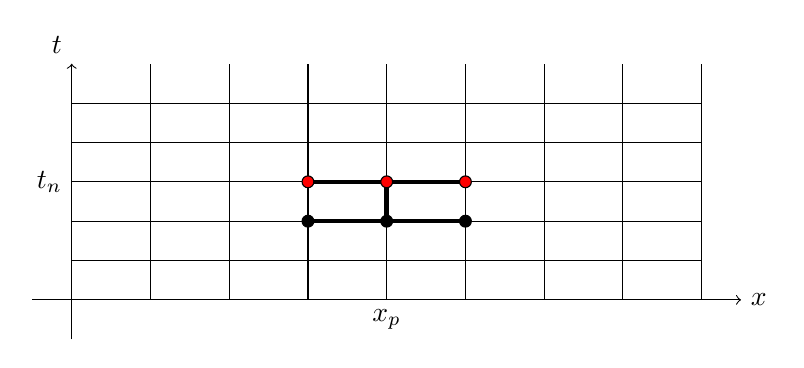
\begin{tikzpicture}[scale=0.5]
\draw[->] (-1,0) -- (17,0);
\node[right] at (17,0) {$x$};
\node[below] at (8,0) {$x_p$};
\draw[->] (0,-1) -- (0,6);
\node[above left] at (0,6) {$t$};
\node[left] at (0,3) {$t_n$};
\foreach \x in {2, 4, ..., 16}
    \draw[thin] (\x,0) -- (\x,6);
\foreach \y in {1, ..., 5}
    \draw[thin] (0,\y) -- (16,\y);
\draw[ultra thick] (6,2) -- (8,2) -- (10,2);
\draw[fill] (6,2)  circle (0.15cm);
\draw[fill] (8,2)  circle (0.15cm);
\draw[fill] (10,2) circle (0.15cm);
\draw[ultra thick] (8,2) -- (8,3);
\draw[ultra thick] (6,3) -- (8,3) -- (10,3);
\draw[fill=red] (6,3)  circle (0.15cm);
\draw[fill=red] (8,3)  circle (0.15cm);
\draw[fill=red] (10,3) circle (0.15cm);
\end{tikzpicture}
\end{center}
\end{figure}

This observation leads us to consider the \emph{Crank--Nicolson method} 
for~\eqref{eq: heat ivp 1d}:
\begin{equation}\label{eq: Crank-Nicolson 1d}
\frac{U^n_p-U^{n-1}_p}{\Delta t}
    -a\,\frac{U^{n-1/2}_{p+1}-2U^{n-1/2}_p+U^{n-1/2}_{p-1}}{\Delta x^2}
    =f^{n-1/2}_p
\end{equation}
for $1\le p\le P-1$ and $1\le n\le N$, where we have used the notation
\[
U^{n-1/2}_p=\frac{U^n_p+U^{n-1}_p}{2}\approx u(x_p,t_{n-1/2}),
\]
and, on the right-hand side, 
\[
f^{n-1/2}_p=\frac{f^n_p+f^{n-1}_p}{2}\approx f(x_p,t_{n-1/2})
\quad\text{or}\quad
f^{n-1/2}_p=f(x_p,t_{n-1/2}).
\]
The usual discrete boundary conditions are imposed,
\[
U^n_0=\gamma_0^n\quad\text{and}\quad
U^n_P=\gamma_L^n\quad\text{for $0\le n\le N$,}
\]
along with the usual discrete initial condition
\[
U^0_p=u_{0p}\quad\text{for $1\le p\le P-1$.}
\]
\cref{fig: Crank-Nicolson 1d} shows the stencil for the scheme.
In matrix notation, the Crank--Nicolson method takes the form
\begin{equation}\label{eq: Crank-Nicolson matrix}
\frac{\boldsymbol{U}^n-\boldsymbol{U}^{n-1}}{\Delta t}
    +\boldsymbol{A}\boldsymbol{U}^{n-1/2}=\boldsymbol{f}^{n-1/2}
    +\boldsymbol{g}^{n-1/2},
\end{equation}
where the $(P-1)\times(P-1)$ matrix~$\boldsymbol{A}$ and 
is same as in~\eqref{eq: implicit Euler 1d vector}, with 
\[
\boldsymbol{g}^{n-1/2}=\frac{\boldsymbol{g}(t_n)+\boldsymbol{g}(t_{n-1})}{2}
\quad\text{or}\quad
\boldsymbol{g}^{n-1/2}=\boldsymbol{g}(t_{n-1/2}),
\]
for $\boldsymbol{g}(t)$ as in~\eqref{eq: U f g semidiscrete 1d}.

Multiplying both sides of~\eqref{eq: Crank-Nicolson matrix} by~$\Delta t$, we 
find that
\[
\boldsymbol{U}^n-\boldsymbol{U}^{n-1}
    +\tfrac12\Delta t\,\boldsymbol{A}(\boldsymbol{U}^n+\boldsymbol{U}^{n-1})
    =\Delta t\,\bigl(\boldsymbol{f}^{n-1/2}+\boldsymbol{g}^{n-1/2}\bigr)
\]
which yields linear system that must be solved at the $n$th time step,
\[
\bigl(\boldsymbol{I}+\tfrac12\Delta t\,\boldsymbol{A}\bigr)\boldsymbol{U}^n=
\bigl(\boldsymbol{I}-\tfrac12\Delta t\,\boldsymbol{A}\bigr)\boldsymbol{U}^{n-1}
    +\Delta t\,\bigl(\boldsymbol{f}^{n-1/2}+\boldsymbol{g}^{n-1/2}\bigr).
\]
The local truncation error for the Crank--Nicolson method is defined by
\begin{multline*}
\tau^{n-1/2}_p=f^{n-1/2}_p-\frac{u(x_p,t_n)-u(x_p,t_{n-1})}{\Delta t}
    +\frac{a}{\Delta x^2}\biggl(
    \frac{u(x_{p+1},t_n)+u(x_{p+1},t_{n-1})}{2}\\
    -2\,\frac{u(x_p,t_n)+u(x_p,t_{n-1})}{2}
    +\frac{u(x_{p-1},t_n)+u(x_{p-1},t_{n-1})}{2}\biggr)r.
\end{multline*}
If we choose $f^{n-1/2}_p=f(x_p,t_{n-1/2})$ then
$f^{n-1/2}_p=u_t(x_p,t_{n-1/2})-au_{xx}(x_p,t_{n-1/2)}$ so
\begin{align*}
\tau^{n-1/2}_p
&=\biggl(u_t(x_p,t_{n-1/2})-\frac{u(x_p,t_n)-u(x_p,t_{n-1})}{\Delta t}\biggr)\\
    &\qquad{}+a\biggl(\frac{u_{xx}(x_p,t_n)+u_{xx}(x_p,t_{n-1})}{2}
        -u_{xx}(x_p,t_{n-1/2})\biggr)\\
    &\qquad{}+\frac{a}{2}\biggl(
    \frac{u(x_{p+1},t_n)-2u(x_p,t_n)+u(x_{p-1},t_n)}{\Delta x^2}-u_{xx}(x_p,t_n)
    \biggr)\\
    &\qquad{}+\frac{a}{2}\biggl(
    \frac{u(x_{p+1},t_{n-1})-2u(x_p,t_{n-1})+u(x_{p-1},t_{n-1})}{\Delta x^2}
        -u_{xx}(x_p,t_{n-1})\biggr).
\end{align*}
Applying Theorems \ref{thm: first central diff}~and \ref{thm: average} with 
$h=\tfrac12\Delta t$, and \cref{thm: 2nd central diff} with~$h=\Delta 
x$, we conclude that
\[
|\tau^{n-1/2}_p|
    \le\frac{(\tfrac12\Delta t)^2}{6}\max_{[0,L]\times[0,T]}|u_{ttt}| 
    +a\,\frac{(\tfrac12\Delta t)^2}{2}\max_{[0,L]\times[0,T]}|u_{xxxx}|
    +a\,\frac{\Delta x^2}{12}\max_{[0,L]\times[0,T]}|u_{xxxx}|
\]
and hence $\tau^{n-1/2}_p=O(\Delta t^2+\Delta x^2)$.  It turns out that the 
Crank--Nicolson method is unconditionally stable, and so 
$U^n_p=u(x_p,t_n)+O(\Delta t^2+\Delta x^2)$.  This higher convergence rate in 
time makes the scheme much more practical than either of the Euler methods.

\section{Another maximum principle}


\begin{Exercises}

\exercise
If the solution~$u(x,t)$ of~\eqref{eq: heat ivp 1d} is continuous
at $(x,t)=(0,0)$ and $(L,0)$, then we must have
\[
u_0(0)=u(0,0)=\gamma_0(0)\quad\text{and}\quad
u_0(L)=u(L,t)=\gamma_L(0).
\]
Show that if $u_t$ and $u_{xx}$ are continuous at~$(x,t)=(L,0)$ and $(L,0)$,
then
\[
\gamma_0'(0)-au_0''(0)=f(0,0)
\quad\text{and}\quad
\gamma_L'(0)-au_0''(L)=f(L,0).
\]

\exercise\label{ex: forward diff}
Use \cref{thm: Taylor remainder} to show that that if $f$ is $C^2$ on 
the closed interval~$[x,x+h]$, then
\[
\biggl|f'(x)-\frac{f(x+h)-f(x)}{h}\biggr|
	\le\frac{h}{2}\max_{x\le y\le x+h}|f''(y)|,
\]
and, similarly, if $f$ is $C^2$ on~$[x-h,x]$, then
\[
\biggl|f'(x)-\frac{f(x)-f(x-h)}{h}\biggr|
	\le\frac{h}{2}\max_{x-h\le y\le x}|f''(y)|,
\]

\exercise
Count the numbers of arithmetic operations used in \cref{alg: explicit Euler} 
to compute the explicit Euler solution.
\begin{ans}
About $4NP$~multiplications and $3NP$ additions, not counting the cost of
evaluating $f$ at $(N-1)(P-1)$~grid points, and $\gamma_0$~and $\gamma_L$
at $N$ grid points.
\end{ans}

\exercise
Let $\phi_k(x)=\sin(k\pi x/L)$.
\begin{description}
\item{(i)} Show that 
\[
\phi_k(x_{p+1})+\phi_k(x_{p-1})=\biggl(2\cos\frac{k\pi\,\Delta x}{2}\biggr)\,
	\phi_k(x_p).
\]
\item{(ii)} Deduce that
\[
-\frac{\phi_k(x_{p+1}-2\phi_k(x_p)+\phi_k(x_{p-1})}{\Delta x^2}
	=\Lambda_k\phi_k(x_p)\quad\text{where}\quad
\Lambda_k=\frac{2}{\Delta x^2}\biggl(1-\cos\frac{k\pi\,\Delta x}{L}\biggr).
\]
\item{(iii)} Show
\[
\Lambda_k=\biggl(\frac{2}{\Delta x}\,\sin\frac{k\pi\,\Delta x}{2L}\biggr)^2.
\]
\item{(iv)}
Find $\lambda_k=\lim_{\Delta x\to0}\Lambda_k$ and verify that 
$-\phi_k''=\lambda_k\phi_k$.
\item{(v)}
Suppose that $u_0(x)=\sin(k\pi x/L)$, $f(x,t)\equiv0$ and 
$\gamma_0(t)\equiv 0\equiv\gamma_L(t)$.  Find $R$ such that the explicit
Euler solution is~$U^n_p=R^n\phi_k(x_p)$.
\item{(vi)} Show that if $a\,\Delta t/\Delta x^2\le1/2$ then $-1\le R<1$
and so $|U^n_p|\le1$ for all $n$~and $p$.
\end{description}
\begin{ans}
(iii) $R=1-a\lambda_k\,\Delta t$\quad(iv) $\lambda_k=(k\pi/L)^2$
\end{ans}

\exercise\label{ex: implicit Euler error}
Prove \cref{thm: implicit Euler error} by adapting the proof of 
\cref{thm: explicit Euler error}.

\exercise
Consider the BDF2 (backward differentiation formula, second-order)
scheme for the heat equation,
\[
\frac{3U^n_p-4U^{n-1}_p+U^{n-2}_p}{2\Delta t}
        -\kappa\,\frac{U^n_{p+1}-2U^n_p+U^n_{p-1}}{\Delta x^2}=f^n_p,
\]
where $1\le p\le P-1$ and $2\le n\le N$.  Assume homogenous Dirichlet
boundary conditions,
\[
U^n_0=0=U^n_P\quad\text{for $1\le n\le N$,}
\]
and initial conditions $U^0_p=v(x_p)$ for~$0\le p\le P$.
\begin{description}
\item{(i)} Draw the stencil for the BDF2 scheme.
\item{(ii)} Define the local truncation error~$\tau(x,t)$ for this
scheme and show that $\tau=O(\Delta t^2+\Delta x^2)$.
\item{(iii)} Write the BDF2 scheme in matrix--vector form, and hence
describe the linear system that must be solved at the $n$th time step
for~$2\le n\le N$.
\item{(iv)} To compute $U^n_p$ when~$n=1$, we use the implicit Euler
scheme,
\[
\frac{U^1_p-U^0_p}{\Delta t}
        -\kappa\,\frac{U^1_{p+1}-2U^1_p+U^1_{p-1}}{\Delta x^2}=f^1_p.
\]
Why does the use of this method ensure that
\[
U^1_p=u(x_p,t_1)+O(\Delta t^2+\Delta x^2),
\]
when we saw in lectures that the implicit Euler method is only
first-order accurate in time?  
\end{description}

\end{Exercises}
